\documentclass[14pt]{beamer}
\title[JPL:Java:01]{JPL :: For...Loops}
\author[TS]{TalentSprint}
\institute[L\&D]{Licensed To Skill}
\date{Version 1.0.4}
\usefonttheme{serif}
\usecolortheme{orchid}
\usepackage{bookman}
\usepackage{hyperref}
\usepackage[font={scriptsize,bf}]{caption}
\usepackage[T1]{fontenc}
\usepackage{color}
\usepackage{graphicx}
\usepackage{listings}
\graphicspath{{../../Images/}}
\usepackage{tikz}
\usepackage{amssymb}
%\usepackage{tikz-cd}
\usepackage{color}
\beamertemplateballitem
\usebackgroundtemplate{
\includegraphics[width=\paperwidth]{TS-XP-Logo.jpg}}
\lstset{language=Java,numbers=left, numberstyle=\tiny, basicstyle=\footnotesize, numbersep=10pt, showstringspaces=false, breaklines=true,keepspaces=true, columns=flexible}
\begin{document}

\begin{frame}
  \titlepage
\end{frame}

\begin{frame}{Learning Objectives}
The content in this presentation is aimed at teaching  learners to:
  \begin{itemize}
  \item Write solutions for simple problems needing iterative execution of a set of steps a certain number of times.
  \item Write Java programs using \lstinline!for! loops 
  \end{itemize}
\end{frame}

\begin{frame}[fragile]{For...Loops}
\textbf{Sum of 'n' Numbers}

\vspace{1pc}

\colorbox{white}{10, 7, 232, 44, 8, 526, 49, 64, 98, 12, ..., n}

\hspace{4cm}$\Uparrow$

\hspace{2cm}\colorbox{cyan}{What is the sum?}
\begin{block}{How about the following approach:}
Read number of numbers (n). 

Repeat `n' times.

Read next number (new\_number)

sum\_so\_far = sum\_so\_far + new\_number 

Print sum\_so\_far

\end{block}

\end{frame}

\begin{frame}[fragile]{For...Loops}
\begin{block}{Solution for finding Sum of `n' Numbers}
\begin{lstlisting}[numbers=none]
Read n;

sumSoFar = 0;

for i = 1 to n

Read next number (newNumber)

sumSoFar = sumSoFar + newNumber

print sumSoFar

\end{lstlisting}
\end{block}
\end{frame}

\begin{frame}[fragile]{For...Loops}
\begin{block}{Java Code  to find Sum of `n' Numbers Using - `for' Loop }
\begin{lstlisting}[numbers=none]
public class SumWithFor {
    public static void main(String[] args) {
        int next, count, sumSoFar = 0;
        for (count = 0; count < args.length; count++) {
            next = Integer.parseInt(args[count]);
            sumSoFar += next;
        }
        System.out.println("Sum: " + sumSoFar);
    }
}
\end{lstlisting}
\end{block}
\end{frame}


\begin{frame}{For...Loops}
\begin{minipage}{10cm}
\textbf{java} SumWithFor 2 3 4 2 
\begin{block}{Output}
Sum: 11
\end{block}
\end{minipage}

\vspace{1pc}
\begin{minipage}{4cm}
\tiny
Before entering loop, sumSoFar = 0
\begin{tabular}{| p{1.2cm} | p{2cm} | p{2cm} |}
\hline
\textbf{count} & \textbf{sumSoFar} & \textbf{condition} \\ \hline
0 & 0 & T \\ \hline
1 & 2 & T \\ \hline
2 & 5 & T \\ \hline
3 & 9 & T \\ \hline
4 & 11 & F \\ \hline
\end{tabular}
\end{minipage}
\end{frame}

\begin{frame}[fragile]{For...Loops}
`\lstinline!for!' Statement

\vspace{1pc}
The `\lstinline!for!' statement allows you to repeat execution of a set of statements a specific number of times.
\begin{block}{Syntax of  `for'  Statement:}
\begin{lstlisting}[numbers=none]
for (initialization; termination; increment/decrement) { 
    statement(s);
}  
\end{lstlisting}
\end{block}
\end{frame}

\begin{frame}{For...Loops}
\begin{minipage}{7cm}
Write Java code, using `\lstinline!for!' loop, to find largest number among `n' numbers.
\end{minipage}
\quad
\begin{minipage}{2cm}
 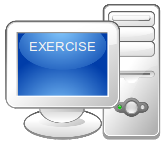
\includegraphics[scale=.5]{exercise.png}
\end{minipage}
\end{frame}

\begin{frame}[fragile]{For...Loops}
\begin{block}{Solution:}
\begin{lstlisting}[numbers=none]
public class LargestWithFor {
    public static void main(String[] args) {  
        int next, count, largestSoFar;  
        for (count=1; count < args.length; count++) {
            next = Integer.parseInt(args[count]);
        }
        System.out.println("Largest: " + largestSoFar);
    }
}
\end{lstlisting}

\end{block}
\end{frame}

\begin{frame}[fragile]{For...Loops}
Find Even or Odd numbers among the numbers from 1 to `n'
\begin{block}{Solution:}
\begin{lstlisting}[numbers=none]
Read n
for x from 1 to n
    if (x % 2 == 0) 
        printf("%d", x , ": is even.");
    else 
        printf("%d", x, ": is odd.");
\end{lstlisting}
\end{block}
\end{frame}

\begin{frame}[fragile]{For...Loops}
\begin{block}{Java Code to Find Odd or Even Numbers:}
\begin{lstlisting}[numbers=none]
 public class EvenNumber {
    public static void main(String[] args) {
        int i;
        int givenNumber = Integer.parseInt(args[0]);
        for (i = 1; i <= givenNumber; i++) {
            if (i % 2 == 0) 
                System.out.println(i + " is even.");
            else
                System.out.println(i + " is odd.");
        }
    }
}
\end{lstlisting}
\end{block}
\end{frame}

\begin{frame}{For...Loops}
\begin{block}{The Problem}
Find if a number is a Prime number or not.
\end{block}
\begin{block}{High Level Solution}
Check if there is a divisor to given number which is other than 1 and itself. If there is, the number is not prime. Otherwise, prime.
\end{block}
\end{frame}

\begin{frame}[fragile]{For...Loops}
\begin{block}{Detailed Solution}
\begin{lstlisting}[numbers=none]
Read the number into n.
for i from 2 to n-1, 
    if n % i = 0, then print ("n not prime").
Print ("n prime");
\end{lstlisting}
\end{block}
\end{frame}

\begin{frame}[fragile]{For...Loops}
\begin{block}{Java Code to Find Prime Numbers:}
\begin{lstlisting}[numbers=none]
public class PrimeNumber {
    public static void main(String[] args) {
        int i;
        int givenNumber = Integer.parseInt(args[0]);
        for (i = 2; i <= givenNumber - 1; i++) {
            if (givenNumber % i == 0) {
                System.out.println (givenNumber + " is not prime.");
                return;
            }
        }
        System.out.println(givenNumber + " is prime");
    }
}
\end{lstlisting}
\end{block}
\end{frame}

\begin{frame}{For...Loops}
\begin{minipage}{7cm}
Write Java code for printing first `n' odd numbers.
\end{minipage}
\quad
\begin{minipage}{2cm}
 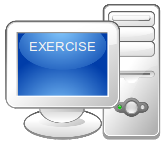
\includegraphics[scale=.5]{exercise.png}
\end{minipage}
\end{frame}

\begin{frame}{For...Loops}
 \begin{figure}[H]
 \begin{center}
   
\includegraphics[scale=.3]{qa.png}   
 \end{center}
  \end{figure}
\end{frame}



\end{document}

